\chapter{実験結果と考察}

\section{評価方法}
%入力希釈木の変形操作を用いた場合と用いなかった場合での希釈木のマッピング結果を比較して,
%入力希釈木の変形操作のFlushing操作を減少させる効果を評価する.
提案手法における希釈木の変形操作の評価を行うため,変形操作を行った希釈木と変形操作を行わなかった希釈木のそれぞれを入力として,
PMD上での液滴移動のない混合手順の生成を行った.
その後,それぞれの希釈木に対する混合手順において必要となったフラッシングの回数を比較することで,
希釈木の変形操作によるフラッシングの回数の削減率を求め,希釈木の変形操作の有効性を測った.

具体的な評価方法を述べる.
まず,高さ3,高さ4,高さ5のそれぞれの高さの希釈木を,500個ずつランダムに生成した.
その後,それぞれの高さごとの,すべての希釈木に関して,変形操作を行った希釈木と変形操作を行わなかった希釈木のそれぞれを入力とし,
PMD上での液滴移動のない混合手順の生成を行った.
これによって得られた混合手順の内,
変形操作を行った希釈木と変形操作を行わなかった希釈木の,どちらを入力として得られた混合手順も,
必要となるフラッシング回数が1以上だった場合のみ,希釈木の変形操作によるフラッシング回数の削減率を求めた.
そして,それぞれの高さごとにこの削減率の平均を求め,希釈木の変形操作のフラッシング回数の削減における有効性を求めた.

\section{実験結果と考察}
%実験結果を表で載せる.実験結果から分かることや考察を述べる.
\begin{table}[tbp]
\caption{分析結果1}
\begin{tabular}{l|r|r|r} \Hline
\multicolumn{1}{l|}{希釈木の高さ}& \multicolumn{1}{l|}{2$\times$2ミキサー平均個数} &  \multicolumn{1}{l|}{2$\times$3ミキサー平均個数} & \multicolumn{1}{l}{フラッシングの削減率($\%$)} \\\hline\hline
3  & 3.26 & 4.16 & -0.29 \\\hline
4  & 7.17&9.06&2.92  \\\hline
5  & 13.37&17.67&5.18  \\\hline
\end{tabular}
\label{table:result}
\end{table}

\begin{figure}[tbp]
 \centering 
    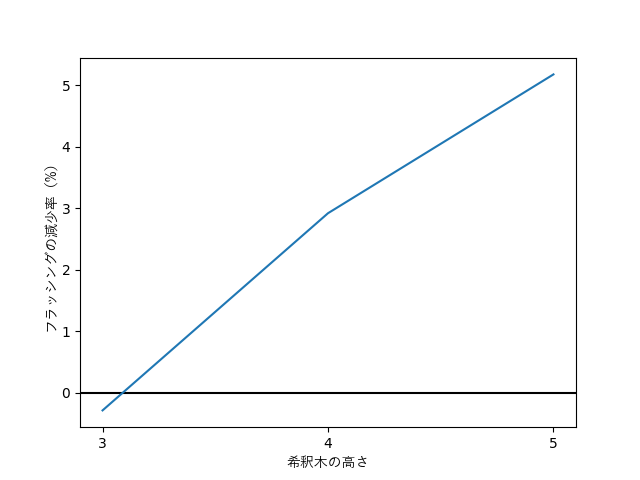
\includegraphics[scale=1.0]{img/decreasement.png}
 \caption{3,4,5のそれぞれの高さを持つ希釈木での変形操作による,フラッシングの平均削減率}\label{fig:graph}
\end{figure}
